% Source : http://tex.stackexchange.com/questions/46354/environment-for-step-by-step-modification-of-graphics

\documentclass{beamer}
	\usepackage{tikz}


\begin{document}
	\begin{frame}[fragile]%
		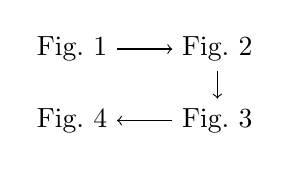
\begin{tikzpicture}
			\draw node(1) {Fig.~1};
			% The onslides are needed or your picture will jump.
			\onslide<2->{
				\draw (1.east)  + (+2em,0) node(2)[anchor=west] {Fig.~2};
			}
			\onslide<3->{
				\draw (2.south) + (0,-1em) node(3)[anchor=north] {Fig.~3};
			}
			\onslide<4->{
				\draw (1.south|-3) node(4) {Fig.~4};
			}
			\draw<2->[->] (1) -- (2);
			\draw<3->[->] (2) -- (3);
			\draw<4->[->] (3) -- (4);
		\end{tikzpicture}
	\end{frame}
\end{document}
